%!TEX root = syntheyes15.tex

\section{Rendering Photo-Realistic Images}

\commentA{past tense}

% needs rewording
In this section we first describe how we rendered our eye-region models, then we briefly describe how we use image-based lighting \cite{debevec2002image} to model a wide range of realistic lighting conditions, and then finally discuss the details of our rendering setup.

% not sure if its worthwhile trying to formally parameterize the rendering model in the paper
% might be simpler to just use words?
For a chosen eye-region model configuration, each rendered image is determined by parameters $(\mathbf{c}, \mathbf{g}, L)$: 3D camera position $\mathbf{c}$; 3D gaze vector $\mathbf{g}$; and lighting environment $L$.
As shown in \autoref{fig:cam_pos}, camera positions $\mathbf{c}$ were chosen by iterating over spherical coordinates $(r, \theta, \phi)$, centered around the eyeball center.
We used an orthographic camera, as this simulates an eye region-of-interest being cropped from a wide-angle camera image, so we set $r\!=\!1$ for convenience.
At each camera position $\mathbf{c}$, we rendered multiple images with different gaze vectors to simulate the eye looking in different directions.
Examples with fixed $L$ are shown in \autoref{fig:cam_pos_example_renders}.
Gaze vectors $\mathbf{g}$ were chosen by first pointing the eye directly at the camera (simulating eye-contact), and then modifying the eyeball's pitch ($\alpha$) and yaw ($\beta$) angles over a chosen range.
%
A consequence of this approach is the possibility of rendering ``unhelpful'' images that either simulate impossible scenarios or are not useful for training.
To avoid violating anatomical constraints, we only rendered images for valid eyeball rotations $|\alpha|\!\leq\!25^{\circ}$ and $|\beta|\!\leq\!35^{\circ}$ \cite{MIL-STD-1472G}.
Before rendering, we also verified that the projected 2D pupil center in the image was within the 2D polygon of the eyelid landmarks -- this prevented us from rendering images where too little of the iris was visible.

\begin{figure}
    \centering
    \begin{subfigure}[t]{0.48\columnwidth}
        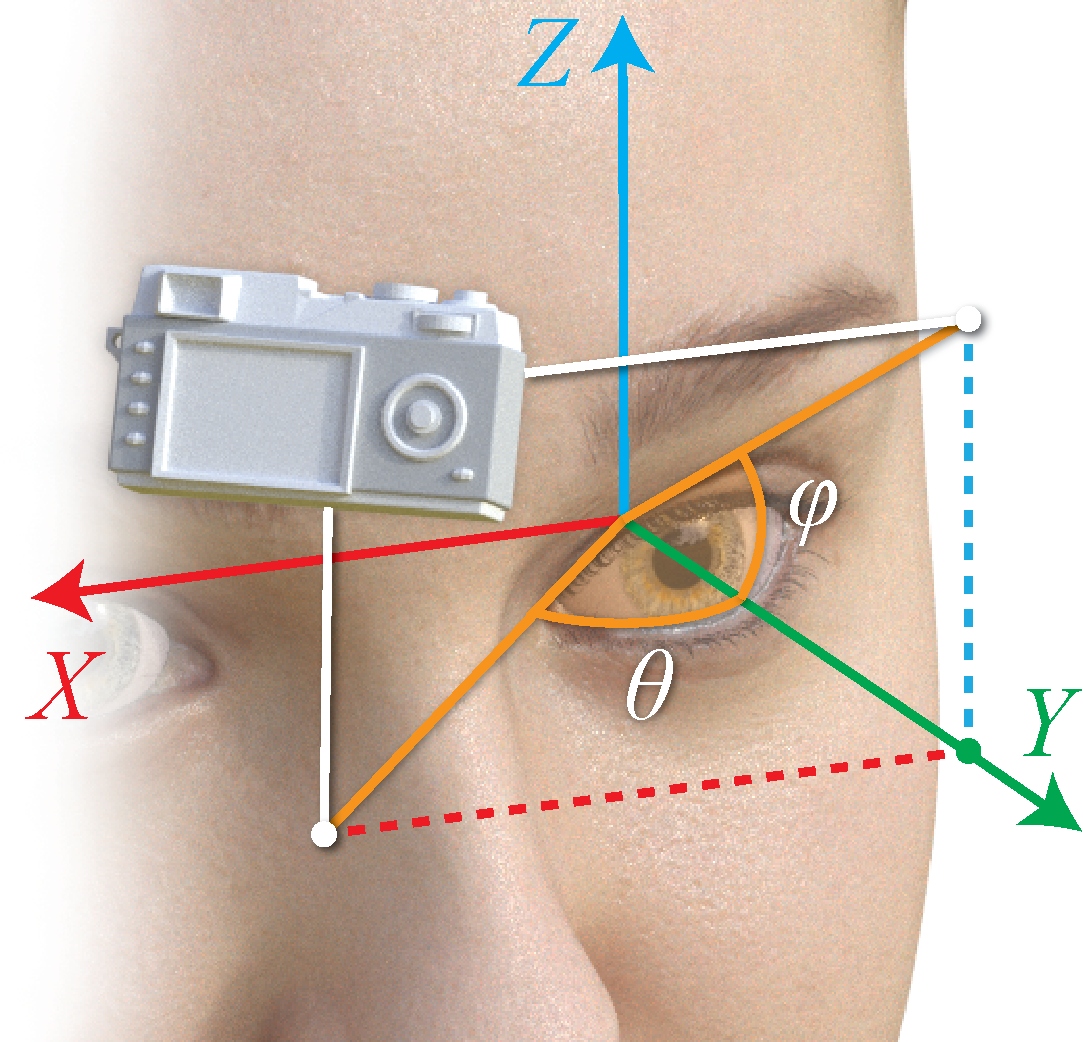
\includegraphics[width=\textwidth]{camera_position}
        \caption{The camera is positioned using spherical coordinates}
        \label{fig:cam_pos_spher_coords}
    \end{subfigure}
    \hfill
    \begin{subfigure}[t]{0.48\columnwidth}
        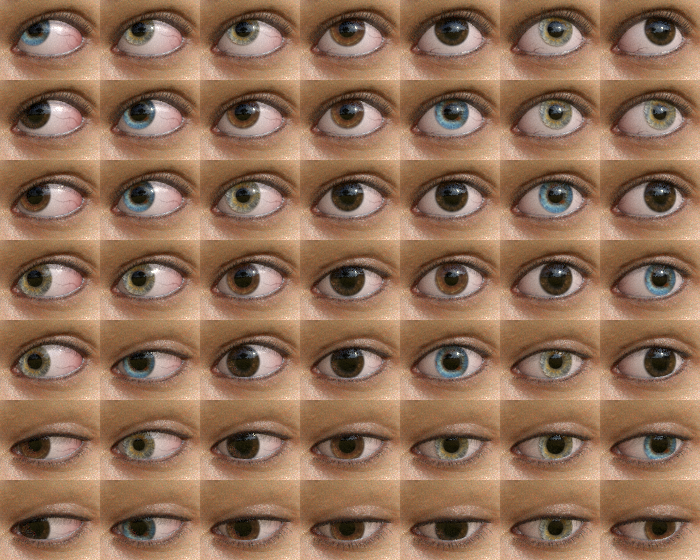
\includegraphics[width=\textwidth]{camera_pos_sample_renders_7x7}
        \caption{At each camera position, we render many gaze directions}
        \label{fig:cam_pos_example_renders}
    \end{subfigure}
    \caption{\ref{fig:cam_pos_spher_coords} shows how we position the camera to simulate changes in head pose. At each camera position, we render many eye images (\ref{fig:cam_pos_example_renders}) by posing the eyeball model.}
    \label{fig:cam_pos}
\end{figure}

\subsection{Lighting the Model}

One of the main challenges in eye tracking is illumination invariance -- a good system should be able to track gaze under a range of real-life lighting conditions.
We realistically illuminate our eye-model using \emph{image-based lighting}, a technique where high dynamic range (HDR) panoramic images are used to provide light in a scene \cite{debevec2002image}.
This works by photographically capturing omni-directional light information and storing it in a texture which is projected onto a sphere around the object.
When a ray hits that texture during rendering, it takes that texture's pixel value as light intensity.
At render time we randomly chose one of four freely available HDR environment images to simulate a range of different lighting conditions (see \autoref{fig:environment_maps}) \cite{AdaptiveSamplesHDR}.
Each environment image is then randomly rotated to simulate a continuous range of head-pose within each environment. As shown in \autoref{fig:env_map_imgs_examples}, we can simulate a wide range of different appearances with only a single environment map.

\begin{figure}

    \begin{subfigure}[t]{\columnwidth}
        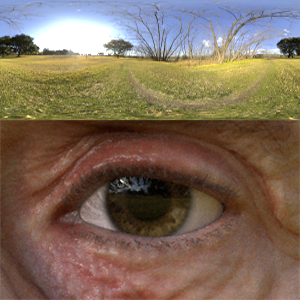
\includegraphics[width=0.24\textwidth]{fig_env_1} \hfill
    	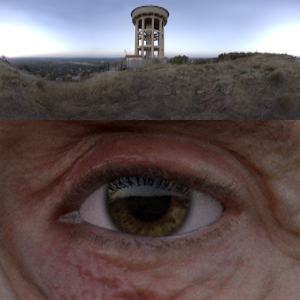
\includegraphics[width=0.24\textwidth]{fig_env_2} \hfill
        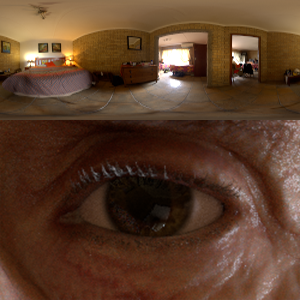
\includegraphics[width=0.24\textwidth]{fig_env_3} \hfill
    	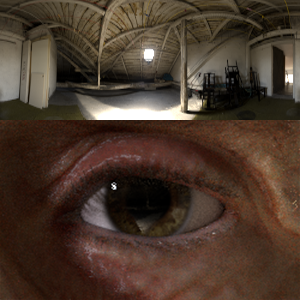
\includegraphics[width=0.24\textwidth]{fig_env_4}
	    \caption{The four HDR environment maps we use for realistic lighting: bright/cloudy outdoors, and bright/dark indoors}
    \end{subfigure}
    \par \medskip
    \begin{subfigure}[t]{0.48\columnwidth}
        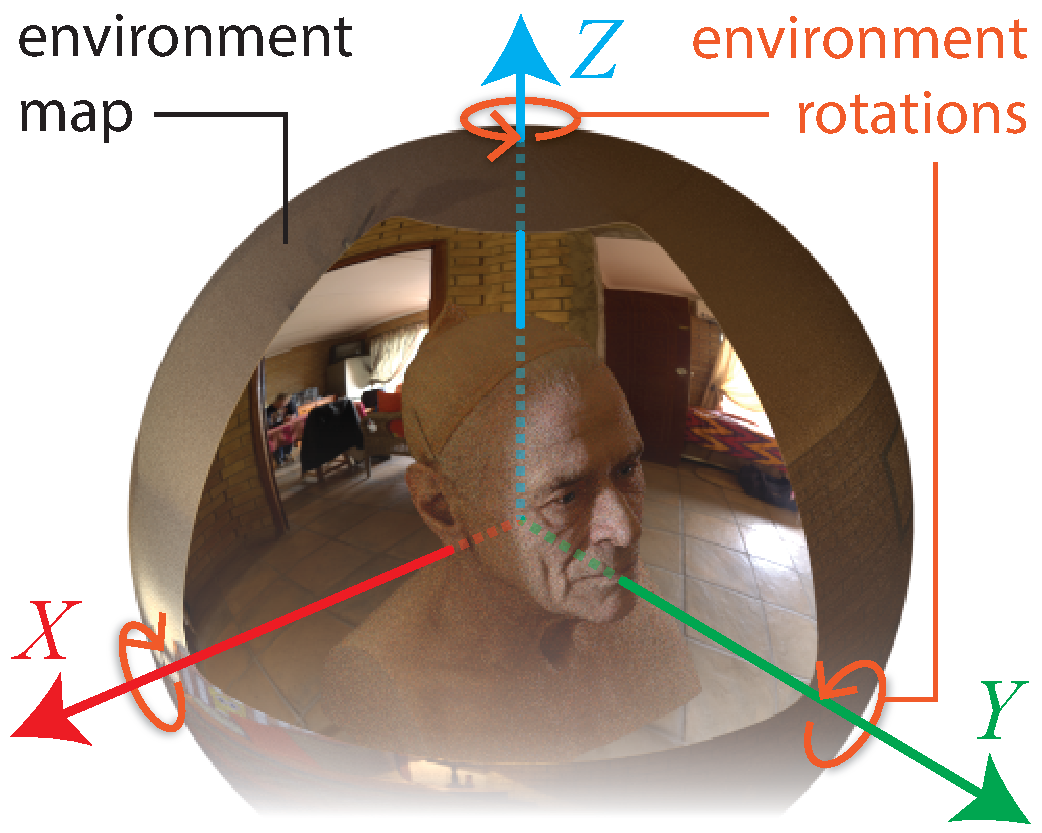
\includegraphics[width=\textwidth]{env_explain_5x4}
    	\caption{we rotate the environment map}
    \end{subfigure}%
    \hfill
    \begin{subfigure}[t]{0.48\columnwidth}
        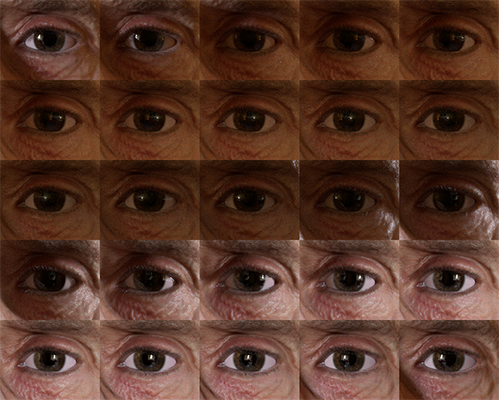
\includegraphics[width=\textwidth]{env_variation}
        \caption{Example images rendered using a single environment map, rotated about the Z-axis.}
        \label{fig:env_map_imgs_examples}
    \end{subfigure}
    \caption{Appearance variation from lighting is modelled with poseable high dynamic range environment maps \cite{debevec2002image}.}
    \label{fig:environment_maps}
\end{figure}

\subsection{Computational Setup}

% this whole section will be reworded

We can rapidly generate diverse datasets much faster than manual collection and annotation.

We use Blender's inbuilt Cycles path-tracing engine for rendering \commentE{CITE}. This physically correct Monte Carlo method integrates over light rays that hit a surface, and stochastically calculates how much of it reaches a pixel in the camera. Though it requires a large number of rays, a GPU solution ...

When rendering a $120\!\times\!80$ eye-region image, it took 5 seconds on average using a commodity GPU (Nvidia GTX660). A dataset for a single eye-region model can be rendered in several hours, so it can take several days to render the entire dataset of ten models. This is much faster than the months taken for traditional data collection approaches \cite{zhang15_cvpr}.